%! Author = giaco
%! Date = 16/05/2024

\chapter{Background}
\label{sec:background}
In this chapter, we provide a brief overview of the main concepts that are necessary to understand the work presented in this thesis.
First of all, we start by introducing the concept of Machine Learning (ML) and Deep Learning (DL) in~\ref{sec:machine_learning}.
Then, in~\ref{sec:rl} we will talk in depth about one specific kind of learning, i.e.\ Reinforcement Learning, which is instead the main focus of this work, and we will talk also about Deep Reinforcement Learning (DRL).

\section{Machine Learning}
\label{sec:machine_learning}
%inserire immagine AI-ML-DL
% prendi immagini da qui https://www.geeksforgeeks.org/types-of-machine-learning/

Machine Learning, Fig. \ref{fig:ml_hierarchy}, is the branch of Artificial Intelligence that focuses on developing models and algorithms that let computers learn from data and improve from previous experience without being explicitly programmed for every task.
In simple words, ML teaches the systems to think and understand like humans by learning from the data.
ML finds application in many fields, including natural language processing, computer vision, speech recognition, email filtering, medicine, and many more

There are several types of ML family of algorithms, each with its own characteristics and applications.
Some of the main types are Supervised Learning, Unsupervised Learning, Self-Supervised Learning, and finally Reinforcement Learning, Fig.\ref{fig:ml_types}
A subset of ML is Deep Learning, which focuses on training neural networks with many layers.

We will talk about the different kinds of learning algorithms and DL in the following subsection, while since RL is the focus of this work we will dedicate a proper section.





\begin{figure}[ht]
    \begin{subfigure}[b]{0.45\textwidth}
        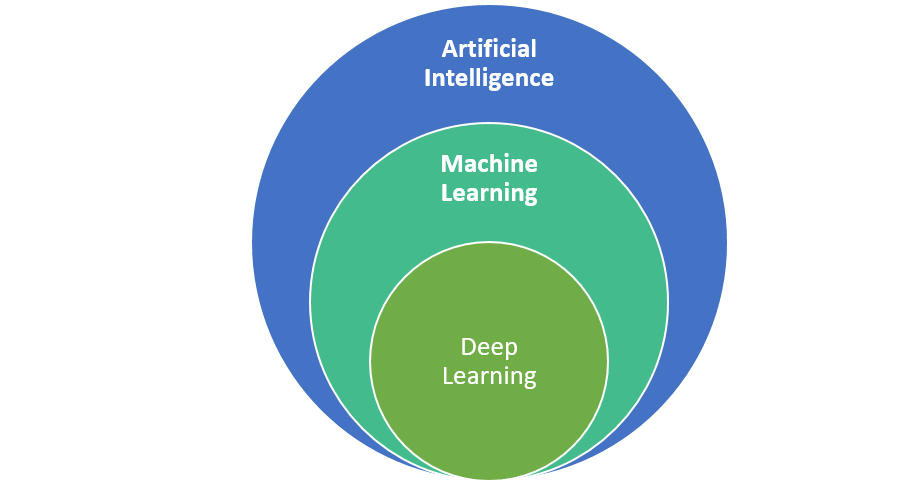
\includegraphics[width=\textwidth]{images/background/ai_ml_dl}
        \caption{\texttt{Artificial Intelligence hierarchy.}}
        \label{fig:ml_hierarchy}
    \end{subfigure}
    \hfill
    \begin{subfigure}[b]{0.45\textwidth}
        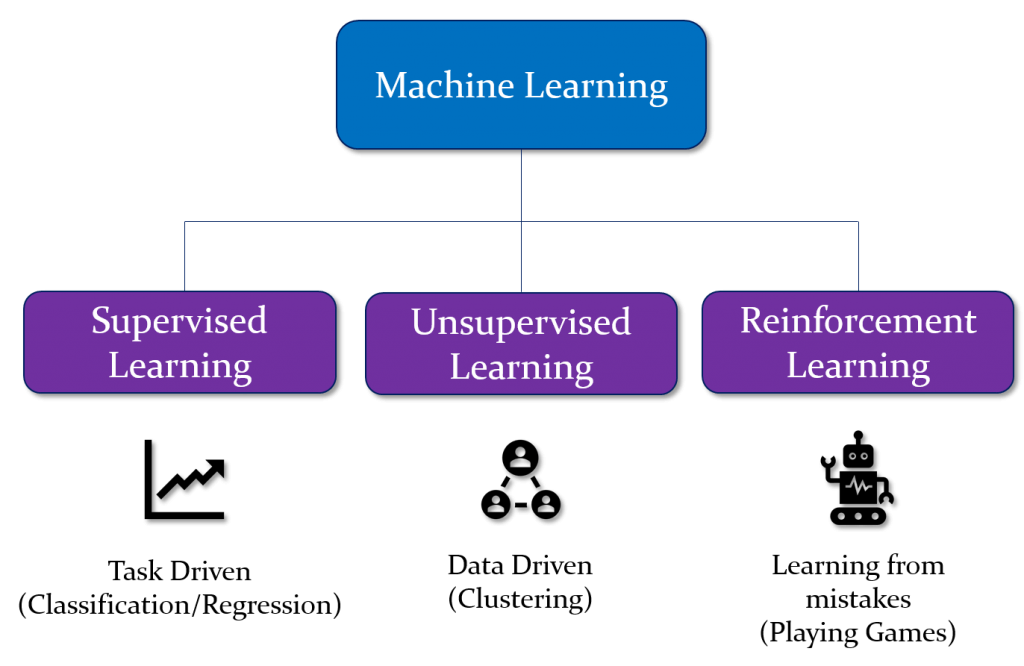
\includegraphics[width=\textwidth]{images/background/ML_Types}
        \caption{\texttt{Some Families of ML algorithms.}}
        \label{fig:ml_types}
    \end{subfigure}
    \hfill
    
\end{figure}








\subsubsection{Supervised Learning}
\label{subsubsec:supervised_ml}
%insert citation of examples of supervised learning?
Supervised Learning is a type of ML where the model is trained on a labeled dataset.
In this context, \textit{labeled} means that each training example is paired with an output label.
The goal of supervised learning is to learn a mapping from inputs to outputs that can be used to predict the output for new, unseen inputs.


There are two main categories of supervised learning that are:
\begin{itemize}
    \item Classification - The goal is to predict a discrete label.
    For example, classifying emails as spam or not spam, or recognizing handwritten digits.
    Classification algorithms learn to map the input features to one of the predefined classes.

    \item Regression - The goal is to predict a continuous value.
    For example, predicting the price of a house given its features, or the temperature for a given day.
    Regression algorithms learn to map the input features to a continuous numerical value.

\end{itemize}

%advantages and disadvantages
Supervised Learning models can have high accuracy as they are trained on labeled data. Also, they can be used as pre-trained models, which saves time and resources when developing new models from scratch.
They have some limitations though, in fact, sometimes they need a huge amount of data to perform well and they may struggle with unseen or unexpected patterns that are not present in the training data. Finally, they can be time-consuming when in the presence of a huge amount of data in the training set.

\subsubsection{Unsupervised Learning}
\label{subsubsec:unsupervised_ml}
Unsupervised learning is a type of ML technique in which an algorithm discovers patterns and relationships using unlabeled data.
Unlike supervised learning, unsupervised learning doesn’t involve providing the algorithm with labeled target outputs.
The primary goal of Unsupervised learning is often to discover hidden patterns, similarities, or clusters within the data, which can then be used for various purposes, such as data exploration, visualization, dimensionality reduction, and more.


The main categories of unsupervised learning are:
\begin{itemize}
    \item Clustering - This is the process of grouping data points into clusters based on their similarities.

    \item Association Rule learning - It is a method used for finding relationships between variables in a large database. A typical example of the Association Rule is the Market Basket Analysis which determines the set of items that occur together like people who buy a specific item also tend to purchase another item.

\end{itemize}


%advantages and disadvantages
Unsupervised Learning helps discover hidden patterns and relationships when labels for data are not available.
Without using labels though, it may be difficult to predict the quality of the model's output.





\subsubsection{Self-Supervised Machine Learning}
\label{sec:semisupervised_ml}
Self-supervised learning is a type of ML technique that falls in between supervised and unsupervised learning.
When in presence of a large amount of unlabeled data, self-supervised learning can be used to learn useful representations of the data.
In fact, it consists of pre-training a model using unlabelled data and generating data labels automatically. Then in the second phase, the algorithm uses the high-confidence data labels among those generated to train the model again in subsequent iterations, like the supervised learning method. The only difference is that the data labels used as ground truth in every iteration are changed.

Self-supervised learning is a powerful technique that can be used to learn useful representations of the data, and it can be used as a pre-training step for supervised learning tasks.
Self-supervised learning models were used in the development of this thesis as we will see in section INSERT.



\subsubsection{Deep Learning}
\label{sec:dl}
Deep Learning is a subfield of ML that, in the last years, has gained a lot of attention and has been successful in many fields.
It can be used in supervised, unsupervised, and self-supervised learning tasks, and it focuses on training neural networks with many layers, where each layer is responsible for extracting features from the input data at different levels of abstraction.

Specifically, a Neural Network (NN) is an Artificial Intelligence method that is inspired by the way the human brain works.
Every NN, consists of layers of interconnected nodes, which are called neurons.
A neuron is a computational unit that takes multiple inputs, multiplies them by weights, and sums them up, and applies an activation function to produce an output.
Activation functions are used to decide whether a neuron should be activated or not based on the weighted sum of the inputs.
They can be linear or non-linear functions, and they introduce non-linearity in the model, which allows the model to learn more complex patterns in the data rather than linear ones.
Examples of non-linear activation functions are the sigmoid, the ReLU, and the tanh function.

In specific, the computation of a neuron can be expressed as:

\begin{equation}
    y = f(\sum_{i=1}^{n} w_i x_i + b)\label{eq:neuron}
\end{equation}

Where $y$ is the output of the neuron, $f$ is the activation function, $w_i$ are the weights, $x_i$ are the inputs, and $b$ is the bias term.
Fig. \ref{fig:single_neuron} shows a picture of a single neuron.
It is possible to see a NN as a composition of multiple neurons, where the output of one neuron is the input of the next one.
We define Multilayer Perceptron (MLP) as a sequential model that is composed of multiple layers of neurons.
We have an input layer, which is responsible for receiving the input data, one or more hidden layers, that are responsible for processing the data in a way that encodes the information in a latent space, and finally an output layer, which is responsible for producing the output information.
In specific, we talk about feed-forward neural networks, when the information flows from the input layer to the output layer without any feedback connections, and we talk about fully-connected neural networks when each neuron in a layer is connected to every neuron in the next layer.
The mathematical representation of a feed-forward neural network is expressed in Eq. \ref{eq:nn}, while Fig. \ref{fig:nn} shows a picture of a feed-forward neural network.

\begin{equation}
    \hat{y} = f_n(f_{n-1}(\dots f_1(\sum_{i=1}^{n} w_i x_i + b_1) + b_{n-1}) + b_n)\label{eq:nn}
\end{equation}


The process of learning the weights relies on the backpropagation algorithm that consists of two main steps: forward pass and backward pass.

Suppose we are in a supervised learning setting, and we dispose to a dataset of input-output pairs $(x, y)$, where $x$ is the input data, and $y$ is the output data that we refer to as ground-truth.
In the forward pass, the input data is passed through the network, and the output \textit{\hat{y}} is computed.
Then, considering the output of the network, the error is computed using a loss function which is a distance metric and measures the difference between the predicted output and the true output.
A typical loss function is the Mean Squared Error (MSE) which is defined as:

\begin{equation}
    MSE = \frac{1}{n} \sum_{i=1}^{n} (y_i - \hat{y}_i)^2
\end{equation}

The backward pass consists of propagating the error back through the network, from output layer to the input one, and it is responsible for updating the weights to minimize the error between the predicted output and the ground-truth.
Weights are updated using the gradient descent algorithm, which is an optimization method that iteratively updates the weights in the direction of the steepest descent of the loss function.
In neural networks, backpropagation is implemented using the chain rule (of calculus) to compute the gradients of the loss function with respect to the weights.
Chain rule allowed to decompose the computation of the gradient of the loss function with respect to the weights into simpler computations, making the computation of the gradients more efficient and allowing the training of deep neural networks.
%insert figure



In the literature, multi-layered neural networks are referred to as Deep Neural Networks (DNNs), and the process of training them is called Deep Learning (DL).
One of the most successful architectures in deep learning is the Convolutional Neural Network (CNN), which is widely used in computer vision tasks.
CNNs are composed of:
\begin{itemize}
    \item convolutional layers, which applies a set of kernels to the input data to extract features.
    Each kernel extracts a different feature, and the output of a convolutional layer is a set of feature maps.
    \item activation functions, which introduce non-linearity in the model.
    \item pooling layers, which reduce the dimensionality of the data by reducing the size of feature maps.
    A typical example of pooling is the max-pooling, which takes the maximum value in a window of the feature map.
    \item fully connected layers, which takes as input the extracted features and makes the predictions.
\end{itemize}

Fig. \ref{fig:cnn} shows a picture of a CNN architecture.

%talk about feed forward nn vs cnn?

\section{Reinforcement Learning}
\label{sec:rl}
% inserire reward hypothesis?
Reinforcement Learning is a paradigm of ML works in a way that mimics the trial-and-error learning process that humans use to achieve their goals.
The principle elements that comprise RL are the agent, the environment, and the reward signal.
The agent is the learner that interacts with the environment and RL focuses on training agents to make sequences of decisions in the environment to maximize a scalar reward signal.
In particular, in RL, there is no supervision.
The only feedback that the agent receives is the reward signal that indicates how well it is doing and should be informative enough to let the agent learn the optimal behavior.
Fig. \ref{fig:rl} shows a picture of the RL paradigm.

Environments can be fully observable when the agent has access to the complete state of the environment, or partially observable when the agent has access only to a partial observation of the environment.
Specifically, in the presence of fully observable environments, we formalize the RL problem as a Markov Decision Process (MDP), which is a tuple $(S, A, P, R, \gamma)$, where:
\begin{itemize}
    \item $S$ is the set of states that the agent can be in.
    \item $A$ is the set of actions that the agent can take.
    \item $P$ is the transition probability function, which defines the probability of transitioning from one state to another given an action.
    \item $R$ is the reward function, which defines the reward that the agent receives when transitioning from one state to another.
    \item $\gamma$ is the discount factor, which determines the importance of future rewards.
    If it is close to 0, the agent will consider only immediate rewards, while if it is close to 1, the agent will consider future rewards.
\end{itemize}

It is possible to define the return of an agent in an MDP as the sum of discounted reward from a specific timestep t.
In particular:
\begin{equation} \label{eq:return}
    G_t = R_{t+1} + \gamma R_{t+2} + \gamma^2 R_{t+3} + \dots = \sum_{k=0}^{\infty} \gamma^k R_{t+k+1}
\end{equation}

The principal components of an RL agent are three and in order are: the policy $\pi$, the value function $v$, and the model $m$.
The policy defines the behavior of the agent, and it is a mapping from states to actions.
Policy can be deterministic if it maps states to a single action, or stochastic if it maps states to a distribution over actions.
The policy can be represented as a table, a function, or a neural network and in the context of MDPs, the policy is defined as $\pi(a|s) = P(a|s)$, which is the probability of taking action $a$ in state $s$.


The value function estimates the expected return that the agent can achieve starting from a given state and following a given policy $\pi$.
It is used to evaluate how good a state is, and it is defined as:
\begin{equation} \label{eq:value_function}
    v_{\pi}(s) = \E_{\pi}[R_{t+1} + \gamma R_{t+2} + \gamma^2 R_{t+3} + \dots | S_t = s] = \E_{\pi}[G_t | S_t = s]
\end{equation}
This is also called the \textbf{state-value function}.
It exists an equivalent function that estimates the expected return that the agent can achieve starting from a given state, taking a specific action, and then following a given policy $\pi$.
This is called the \textbf{action-value function}, and it is defined in Eq. \ref{eq:action_value_function}.
Value functions too can be represented as tables, functions, or neural networks.

\begin{equation} \label{eq:action_value_function}
    q_{\pi}(s, a) = \E_{\pi}[R_{t+1} + \gamma R_{t+2} + \gamma^2 R_{t+3} + \dots | S_t = s, A_t = a] = \E_{\pi}[G_t | S_t = s, A_t = a]
\end{equation}


The model is used to predict what the environment will do next, so it is a representation of the environment and predicts the next state given current state and action, $P_{s, s'}^a = P(S_{t+1} = s' | S_t = s, A_t = a)$ and predicts the next reward given the current state and action, $R_s^a = \E[R_{t+1} | S_t = s, A_t = a]$.

The concept of learning in RL is based on the \textbf{Bellman Equations}, which form the basis for many RL algorithms and are divided into two main categories: the Bellman Expectation Equations and the Bellman Optimality Equations.
To estimates the goodness of a state, we can use the \textbf{Bellman Expectation Equations} for the state-value function and the action-value function, which provides a recursive relationship between the value of a state and the value of the next state.

Bellman Equation for state-value function is defined in Eq. \ref{eq:bellman_state_value} where the expected return is decomposed into the immediate reward and the discounted value of the next state, and then we marginalize over the actions to obtain the expected value of the state in terms of the action-value function.

\begin{equation} \label{eq:bellman_state_value}
    v_{\pi}(s) = \E_{\pi}[R_{t+1} + \gamma v_{\pi}(S_{t+1}) | S_t = s] = \sum_{a} \pi(a|s)q_{\pi}(s, a)
\end{equation}

Similarly, the Bellman Equation for the action-value function is defined in Eq. \ref{eq:bellman_action_value}, where the expected return is decomposed into the immediate reward and the discounted value of the next state-action pair, and then we marginalize over the next states to obtain the expected value of the action in terms of the state-value function.

\begin{equation} \label{eq:bellman_action_value}
    q_{\pi}(s, a) = \E_{\pi}[R_{t+1} + \gamma q_{\pi}(S_{t+1}, A_{t+1}) | S_t = s, A_t = a] = R_s^a + \gamma \sum_{s'} P_{s, s'}^a v_{\pi}(s')
\end{equation}

Now we notice that the Bellman Equation for the state-value function defined in Eq. \ref{eq:bellman_state_value} can be rewritten substituting the action-value function in it, obtaining:

\begin{equation}
    v_{\pi}(s) = \sum_{a} \pi(a|s)(R_s^a + \gamma \sum_{s'} P_{s, s'}^a v_{\pi}(s'))
\end{equation}

Similarly, the Bellman Equation for the action-value function defined in Eq. \ref{eq:bellman_action_value} can be rewritten substituting the state-value function in it, obtaining:

\begin{equation}
    q_{\pi}(s, a) = R_s^a + \gamma \sum_{s'} P_{s, s'}^a \sum_{a'} \pi(a'|s')q_{\pi}(s', a')
\end{equation}



A policy $\pi$ is defined to be better than or equal to a policy $\pi'$ if its expected return is greater than or equal to that of $\pi'$ for all states.
%In other words pi >= pi'  and only if v_pi(s) >= v_pi'(s) for all s.
There is always at least one policy that is better than or equal to all other policies.
This is an \textit{optimal policy}.
There may be more than one optimal policies, but we denote all the optimal policies by $\pi^*$.
For finding the optimal policy $\pi^*$, we can use the \textbf{Bellman Optimality Equations} both for the state-value function and the action-value function.
Supposing that we have the optimal action-value function $q_*(s, a)$, we can obtain the optimal policy by maximizing over it, i.e.\ choosing the action that maximizes the action-value function in a given state:
\begin{equation}
    \label{eq:optimal_policy}
    \pi^*(a|s) = \begin{cases}
        1 & \text{if } a = \arg\max_{a} q_*(s, a) \\
        0 & \text{otherwise}
    \end{cases}
\end{equation}


So we can define the Bellman Optimality Equation to find the optimal state-value function as follows:
\begin{equation} \label{eq:optimal_state_value}
    v_*(s) = \max_{a} q_*(s, a) = \max_{a} R_{t+1}^a + \gamma \sum_{s'} P_{s, s'}^a v_*(s')
\end{equation}

And the Bellman Optimality Equation to find the optimal action-value function as follows:
\begin{equation} \label{eq:optimal_action_value}
    q_*(s, a) = R_s^a + \gamma \sum_{s'} P_{s, s'}^a v_*(s') = R_s^a + \gamma \sum_{s'} P_{s, s'}^a \max_{a'} q_*(s', a')
\end{equation}

Solving the Bellman Equations means finding the optimal policy, there exist several iterative algorithms to solve them, and they can be divided into two main categories: model-based and model-free.



% model based -> value iteration, policy iteration
% model free -> Q-learning,


%deep reinforcement learning ->
    %-> value function approx DQN
    %-> policy function approx piccola intro
    %-> policy gradient methods


\subsection{Model Based}

\subsection{Model Free}

\subsection{Q Learning}

\subsection{Proximal Policy Optimization}









\section{Deep Reinforcement Learning}
% talk about DQN and PPO

In this section, we talk about the combination of deep learning and reinforcement learning, which is called Deep Reinforcement Learning (DRL).
DRL has been successful in many tasks, including playing video games, controlling robots, and optimizing complex systems.
One of the most successful DRL algorithms is the Deep Q-Network (DQN), which uses a neural network to approximate the Q-function in Q-learning.
DQN has been successful in many tasks, including playing Atari games, and it has been extended to many other algorithms, including Double DQN, Dueling DQN, and Rainbow DQN.
Another successful DRL algorithm is Proximal Policy Optimization (PPO), which uses a neural network to approximate the policy in policy gradient methods.
